\chapter{Multi-fidelity optimization}
% TODO: Multi-fidelity = gray-box optimization
% TODO: Maybe do an overview of the methods and approaches here first

% Introduction - more efficiency by getting early estimates
Even though Bayesian optimization techniques are more sample-efficient compared to a random search, there is another family of approaches that strive to improve the search efficiency further. Instead of training the network until full convergence to obtain the performance metric, multi-fidelity techniques make use of the assumption that a good enough approximation of the final performance can be obtained much faster --- either by stopping early or by training the model on a subset of the training data. This either reduces the computation time or allows the algorithm to evaluate more configurations in the same amount of time. The actual efficiency gain depends on the quality of the intermediate results. The training of neural networks is an inherently noisy process, which makes the problem more challenging. Nevertheless, many approaches successfully exploit multi-fidelity evaluations.

% Fidelity hyperparameter, relationship fidelity vs reliability, rank correlation
Formally, a new hyperparameter $\lambda_{fid}\in [0,1]$ is introduced that allows us to evaluate the function $f(x, \lambda_{fid})$ using just a $\lambda_{fid}$ portion of the full budget (e.g.\ epochs). In most of the literature, the term \textit{budget} is used for specifying the fidelity. Determining the fidelity at which to evaluate the function is the challenging task. Usually, the algorithm has no prior knowledge of the relationship between different fidelities, as well as the reliability of the estimates. That is why most of the multi-fidelity algorithms use some kind of schedule to progressively increase the fidelity hyperparameter.

% Often the algorithms do not try to predict the final performance from low-fidelity evaluations at all. They just compare several configurations at the same fidelity level, hoping the ranking will be similar at a higher fidelity. If a low-fidelity ranking predicts a high-fidelity ranking well, we say that the rank correlation is high. In practice, the reliability of estimates and rank correlation usually gets better as the $\lambda_{fid}$ is increased.

% Don't use multi-fidelity for everything
Finally, we should also note that multi-fidelity techniques are not the universal solution to every hyperparameter optimization problem. If the optimization budget is high, standard random search or Bayesian optimization might perform better, because the partial evaluations can be misleading and good configurations might be discarded too soon. Multi-fidelity techniques usually provide the greatest benefits on a low budget.

\section{Early stopping}

\subsection{Learning curve extrapolation}
% Freeze-thaw paper - extrapolating of learning curves with new kernel (infinite mixture of exponentially decaying basis functions - TODO), Bayesian optimization,
% Authors state there is possible extension to more flexible priors such as spatio-temporal GP with separable covariance
The simplest way to reduce the runtime of an algorithm is to stop the computation before it finishes. Swersky et al.~\cite{swersky2014freeze} noticed that human experts have the ability to assess whether the model will eventually be useful early in the training and developed a method to leverage early stopping. They refer to this method as freeze-thaw Bayesian optimization, because it allows for pausing or aborting the training procedure when the model does not seem promising and resuming the training later if needed. This is combined with the Bayesian optimization framework for hyperparameter search and the authors propose a technique for estimating when to pause and resume training. The algorithm uses an information-theoretic criterion to determine which models to thaw.

% More freeze-thaw and Domhan interpolation of learning curves
Freeze-thaw method relies on the assumption that for many models the training loss roughly follows an exponential decay. Swersky et al.~\cite{swersky2014freeze} developed a new kernel to serve as a prior characterizing the learning curves. This kernel is then used to forecast the final training loss and to provide these estimates to the Bayesian optimization. The kernel was successfully applied to matrix factorization and other problems, but it did not describe the learning curves of deep neural networks well. The same idea was explored by Domhan et al.~\cite{domhan2015speeding}, but with a focus on deep neural networks. They developed a technique for extrapolation of learning curves based on a probabilistic model and used the model to terminate a training run when its performance is most likely going to be worse than the performance of the best model encountered so far. They modeled learning curves using eleven different model families and concluded that even though all of these models capture certain aspects of learning curves, no single model can describe all learning curves by itself. Therefore, they combined the models in a probabilistic framework. Their approach is agnostic to the hyperparameter optimizer and sped up the hyperparameter optimization approximately by a factor of two. Even though the extrapolation of learning curves is a promising approach, it did not catch up.

\subsection{Successive Halving}
% Successive Halving is widespread
 Arguably the most influential approach to multi-fidelity optimization is the Successive Halving algorithm proposed by Jameison and Talwalkar~\cite{jamieson16}. Even though the algorithm is rarely used in its original form, the success of Successive Halving stems from the fact that the algorithm has been used as a basis by many other researchers, presumably for its simplicity and robustness. Successive Halving solves the problem of efficient budget allocation by iteratively increasing the fidelity only for the best candidates. Note that both fidelity and budget denote the same resource in this case.

 % How it works
 The algorithm works in rounds, each round has the same fixed budget $B$ that is uniformly distributed between the candidate solutions. First, it starts with $n$ randomly sampled configurations and the budget is set as $B \leftarrow nb_0$, where $b_0$ is the minimal budget. For simplicity, we can assume that $b_0=1$, which means that in the first round, the budget $B=n$ is uniformly distributed between the $n$ solutions, so each candidate solution is trained for one epoch. After the intermediate results are obtained for all solutions, the algorithm discards the worst half and the first round ends. Since only half of the solutions are left now and the budget for each round is fixed, each solution is allocated twice the budget in the next round. This process is repeated until a single configuration remains. The pseudocode of the generalized algorithm is provided in the Algorithm~\ref{alg:sh}. The only difference is that the generalized algorithm uses a \textit{reduction factor} $\eta$ --- it keeps only $1/\eta$ of the best configurations and the budget is increased by the factor of $\eta$.

 \begin{algorithm}
    \caption{Successive Halving}
    \begin{algorithmic}[1]
    \Statex {\textbf{Input}:} Search space $\mathcal{X}$,\hspace{1mm} number of initial configurations $n$ ,\hspace{1mm} min budget $b_0$,\hspace{1mm} max budget $B$,\hspace{1mm} reduction factor $\eta$.
    \State{$b \leftarrow b_0$}
    \State{Sample $n$ configurations $X \subset \mathcal{X}$ at random.}
    \While{$b \leq B $}
        \For{$x \in X$}
            \State Evaluate x for a budget of b.
        \EndFor
        \State $b \leftarrow \eta b$
        \State Select the $1/\eta$ best performing configurations in $X$ and discard the rest.
    \EndWhile
    \end{algorithmic}
    \label{alg:sh}
\end{algorithm}

% Example computation to illustrate efficiency
To illustrate the efficiency of the algorithm, let us consider a practical example. Suppose we want to optimize the hyperparameters of a network, and we know that it converges within 64 epochs, so we set the maximal budget $B:=64$. We will choose the reduction factor $\eta:=2$, the number of initial configurations $n:=64$, and the minimal budget $b_0:=1$. There will be seven rounds of the algorithm --- with 64, 32, 16, 8, 4, 2, and 1 considered solutions. Each round has a budget of 64, so the total budget spent is 448 epochs. If we have performed a random search and trained the same 64 configurations, a total budget of 4096 would be needed. In this particular case, the search cost was reduced by a factor greater than 9.

% Pros
The algorithm allocates exponentially more resources to more promising configurations to make the search more efficient. A big advantage of Successive Halving is that it is a general algorithm with almost no assumptions on the optimized function. To work well, it only assumes that there is a rank correlation between different fidelities. That is, the ranking of the solutions does not change dramatically from round to round. Fortunately, this is often the case in practice.

% Cons
A theoretical drawback is that the algorithm might never converge. For example, if the best configurations perform poorly in the beginning, then the algorithm discards them before they have the opportunity to converge. A practical downside of the algorithm is that we have to choose its hyperparameters. We should have an estimate of the budgets, but more importantly, we have to choose the number of configurations $n$ in the first round manually. Either we choose large $n$ if we prefer to train a lot of hyperparameter configurations with a smaller training time, or a small $n$, resulting in the exploration of fewer hyperparameter configurations that are allocated a larger budget. This essentially forces us to make the exploration-exploitation trade-off. Finally, the Successive Halving algorithm cannot be parallelized efficiently. After each round, all candidate solutions must be evaluated before a decision can be made and the number of configurations drops each round.

\subsubsection{Asynchronous Successive Halving (ASHA)}
 Extension of the Successive Halving to support massively parallel computing was developed by Li et al.~\cite{li2020system}. Their algorithm also improves several other aspects of the original algorithm, making it more practical to use.

 % How it works - stopping
 ASHA does not have the parameter $n$ that sets the number of initial configurations. Instead, there are $n$ workers that run in parallel. It also does not run in distinct rounds, instead, the different fidelity levels are called \textit{rungs}. There are two variants of the algorithm that differ in how the algorithm behaves when a configuration reaches the next rung --- \textit{stopping} and \textit{promotion}. Upon reaching the next rung, the stopping variant decides immediately whether to stop the run or let it continue. If the trial is among the top $1/\eta$ performing trials currently at the rung, it continues. It is stopped otherwise, and a new configuration is sampled at random for the freed worker. Since at least $\eta$ trials are needed to make the decision, the default action is to continue.

 % How it works - promotion
 The promotion variant can pause and resume trials. When a trial reaches the next rung, it is paused there. Whenever a worker becomes available, all rungs are scanned in descending order for a suitable trial to resume. If a paused run that is in the top $1/\eta$ rung's trials is found, it is promoted and the training continues until the next rung. If no trial to be promoted is found in any of the rungs, a new trial is randomly sampled and starts running.

 % Benefits
 ASHA offers several advantages over Successive Halving. The first is that the number of configurations and rung sizes are not fixed. The algorithm can run for as long as the computational budget allows, adding new configurations as required without any limit. ASHA is also designed for good anytime performance, which is achieved by the promotion and stopping policies. The trials are pushed to finish as soon as possible. As a consequence, the delay until at least one trial is fully finished is reduced, and promising trials do not have to wait for all the other trials to get to the same rung. The anytime performance should be better even if just one worker is available.


\subsection{Hyperband}
% Introduction
The Hyperband algorithm, developed by Li et al.~\cite{li2018hyperband}, is another extension of the Successive Halving algorithm. It is also a pure early-stopping algorithm. The authors suggested extending it with Bayesian optimization but left it for future work. Instead, they focused on the deficiencies of the Successive Halving, namely its reliance on well-chosen hyperparameters. That is probably why the Hyperband became so popular among researchers as well as in the open-source community in hyperparameter optimization frameworks.

% What problem Hyperband tries to solve - the n vs B/n problem
Recall that the Successive Halving needed $n$, the number of configurations to consider, to be determined beforehand by the user. The authors of the Hyperband paper call it ``the $n$ versus $B/n$ problem''. Given some finite budget $B$, the algorithm has to allocate the resources to $n$ configurations, allocating $B/n$ resources on average across the configurations. Therefore, the more configurations the algorithm considers, the less resources per configuration can be allocated on average. Using an example, they illustrate why the optimal choice of $n$ depends mainly on how hard is it to distinguish similarly performing hyperparameter configurations from each other. Because we do not usually have this information, the optimal setting is not known in advance. We include the example because we think it illustrates a general problem that all hyperparameter optimization algorithms face.

% n vs B/n example
The intermediate losses are noisy, so we have to account for the uncertainty. We bound this uncertainty by the maximum deviation of the intermediate losses from the final loss, which the authors of the paper call the envelope (see Figure~\ref{fig:envelopes}). Ideally, we would wait until the envelopes do not overlap. That is, if the final losses are $l_1$ and $l_2$, and the width of the envelopes is less than $l_2-l_1$, then the intermediate losses are guaranteed to be less than $\frac{l_2-l_1}{2}$ from the final losses. From this example we observe that more resources are needed to distinguish two configurations if the envelopes are wider (the losses are more noisy), or if the terminal losses are closer together. The choice of $n$ also places an upper bound on the execution time of a single configuration. Therefore, by choosing $n$ that is too large, there might not be enough time for the best configurations to converge, and we might select a worse hyperparameter configuration as a result.

\begin{figure}
    \centering
    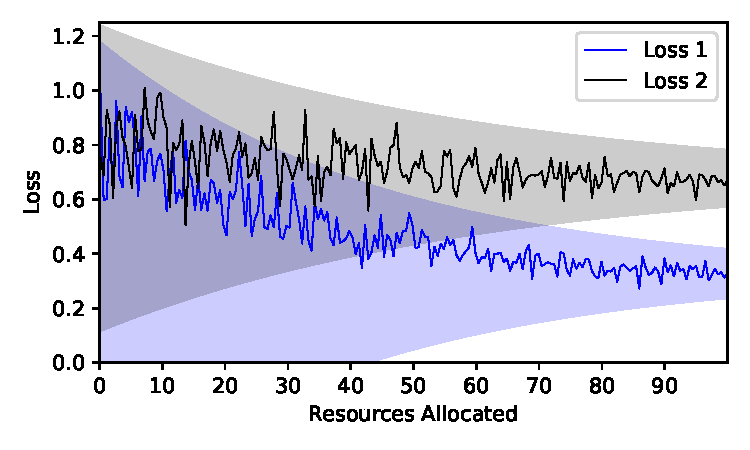
\includegraphics[scale=0.75]{img/loss_envelopes.pdf}
    \caption{An illustration of two loss functions and their envelopes as the shaded area.}
    \label{fig:envelopes}
\end{figure}

% TODO: Is the description of Hyperband correct - HB brackets - how many Successive Halving is run inside of one HB bracket?

% How it solves it the problem
The Hyperband addresses the $n$ versus $B/n$ trade-off by considering several possible values of $n$ for a fixed budget $B$ and running the Successive Halving algorithm several times with different values of $n$. The authors call one run of Successive Halving within Hyperband a \textit{bracket}. Each bracket is designed to use approximately $B$ total resources. With each value of $n$ a minimum resource $r$ is associated that specifies the minimum resource allocated to each configuration. We have called the same parameter $b_0$ in the description of the Successive Halving algorithm. A larger value of $n$ corresponds to a smaller $r$, which in turn results in more aggressive early-stopping. An additional advantage of resetting the search is that Hyperband is hedging against bad instantiations of the randomly sampled configurations and their initialization.
%  since the same amount of computational resources is distributed between more hyperparameter configurations

% Description of the algorithm
Now we describe the Hyperband in greater detail as presented in Algorithm~\ref{alg:hyperband}. In order to run the Hyperband, we need to specify two parameters. First, the maximum amount of resources that can be allocated to a single configuration $R$, and second, the reduction factor $\eta$ that we have already seen in the Successive Halving algorithm. First, the algorithm computes the number of brackets $s_{max}$ from the parameters and the budget it spends per bracket $B$. After the number of brackets is determined, the outer loop iterates over the brackets (line 1). The iteration goes from the most aggressive exploratory bracket (the most initial configurations and Successive Halving rounds) to the bracket with just a single Successive Halving iteration, which is equivalent to a random search. For each bracket, the number of initial configurations $n$ is calculated, as well as the minimal resources spent per configuration $r$ (line 2), so that the bracket spends approximately $B$ resources. The configurations are sampled at random on line 3. The inner loop within the bracket runs standard Successive Halving for the number of iterations given by the bracket (line 4). Inside the Successive Halving loop, we explicitly compute the number of configurations considered in $i$-th iteration as $n_i$ (line 5), as well as the budget $r_i$ that the configurations are trained to (line 6). Then the configurations are evaluated and $ \lfloor n_i/\eta \rfloor$ configurations with the best metric values are kept in $X$, while the rest is removed from the set (lines 7--9).

\begin{algorithm}
    \caption{Hyperband}
    \begin{algorithmic}[1]
    \Statex {\textbf{Input}:} Search space $\mathcal{X}$,\hspace{1mm} maximum resource $R$,\hspace{1mm} reduction factor $\eta$.
    \Statex {\textbf{Initialization}:} $s_{max} = \lfloor log_\eta (R) \rfloor , B=(s_{max}+1)R$
    \For{$s\in \{ s_{max}, s_{max}-1,\ldots ,0 \}$}
    \Comment{Hyperband brackets}
        \State{$n=\lceil \frac{B}{R}\frac{\eta^s}{(s+1)}\rceil, r=R\eta^{-s}$.}
        \State{Sample $n$ configurations $X \subset \mathcal{X}$ at random.}
        \Comment{Start of Successive Halving}
        \For{$i \in \{ 0,\ldots , s \} $}
            \State{$n_i= \lfloor n\eta^{-i} \rfloor$}
            \State{$r_i=r\eta^{i}$}
            \For{$x \in X$}
                \State Evaluate x for a budget of $r_i$.
            \EndFor
        \State Select the $\lfloor n_i/\eta \rfloor $ best performing configurations in $X$.
        \EndFor
    \EndFor
    \State \Return {Configuration with the smallest intermediate loss.}
    \end{algorithmic}
    \label{alg:hyperband}
\end{algorithm}

% Implications
Since the maximum resource parameter $R$ to spend on a single configuration is largely specified by the task, the only parameter left is the reduction factor. Even the reduction factor does not give us much freedom for tuning, which is generally seen as an advantage. We can either use the default value $\eta=3$, or we could opt for a little less or a little more aggressive early stopping by setting it to 2, or 4, respectively. It might also be seen as an advantage or as a disadvantage that the number of resources one run of the Hyperband spends is largely fixed, except for the little room that the parameters give us. As a consequence, the authors recommend running the Hyperband repeatedly if the budget allows it.
%From a practical perspective, it might be helpful to know how much budget one run of the Hyperband uses. For example, if we choose $27\leq R<81$ and keep the reduction factor on the default value, the Hyperband will use four brackets. From the number of brackets, we could compute the budget for one run of the Hyperband.

% Hyperband benchmarks
In the publication~\cite{li2018hyperband}, the authors compare the Hyperband algorithm to three Bayesian optimization algorithms (with TPE, Random Forest, and Gaussian Process as a surrogate) on CIFAR-10, rotated MNIST and SVHN datasets. They also include random search and 2x-random search as a baseline. The Hyperband consistently outperformed other algorithms at the beginning of the search. As the search progressed to spending the whole budget, the differences were only small between the methods.

\subsection{Model-based algorithms}
% BOHB - their desiderata are nice, might state them in the introduction
% BOHB is often said to be SOTA algorithm in follow-up research, maybe I should highlight its importance and write more about it.
%\subsubsection{BOHB}
\subsubsection{Hyperband extensions}
The drawback of Hyperband is that it does not scale well into larger budgets and random search starts to close the gap. Falkner et al.~\cite{falkner2018bohb} proposed a new algorithm BOHB to fix this. They combine Hyperband with Bayesian optimization to complement each other. Bayesian optimization needs a few initial trials to gather enough data to fit the surrogate model, so a few iterations of random search are performed at the beginning. This is where the strong low-budget performance of Hyperband is used. On the other hand, a well-fitted Bayesian optimization model provides better suggestions later in the tuning process. The Bayesian optimization surrogate BOHB uses is based on TPE, but instead of a hierarchy of one-dimensional KDEs, the authors decided to use a single multidimensional KDE in order to better handle interaction effects between the hyperparameters. The number of randomly sampled configurations is $d+1$ by default, where $d$ is the number of hyperparameters. BOHB always fits the surrogate using the observations on the highest budget possible, as soon as enough observations become available.

% DEHB ~\cite{awad2021dehb}
%\subsubsection{DEHB}

% DEHB overview
Another algorithm extending the Hyperband is the DEHB developed by Awad et al.~\cite{awad2021dehb}, which uses an evolutionary optimization method instead of Bayesian optimization. More specifically, the DE stands for Differential Evolution. The authors claim that the evolutionary approach provides some benefits over Bayesian optimization, such as better handling of discrete dimensions, better scaling into high dimensions, and conceptual simplicity enabling easy implementation.

% DEHB parent pool and differential evolution.
DEHB does not run standard Successive Halving. The only time DEHB samples random configurations is in the first step of the first Hyperband iteration. Instead of sampling, DEHB keeps a \textit{subpopulation} at each budget level which serves the purpose of information transfer between brackets --- every subsequent bracket reuses the subpopulation updated in the previous bracket. The size of each subpopulation is equal to the maximum number of function evaluations Hyperband allocates for the corresponding budget. Information is not transferred only horizontally at a fixed budget level, but also vertically, to a higher budget. The top-performing configurations are not just promoted, instead, they are collected in a \textit{parent pool} associated with a budget. On the next budget level, configurations are selected from the subpopulation of that budget and then modified similarly to differential evolution --- three additional configurations are sampled at random from the parent pool to generate a new mutant vector. Then a crossover operation is performed with the vector selected from the subpopulation and the mutant vector to create a new configuration. This configuration is evaluated and if it performs better than the old, it replaces the old configuration in the subpopulation. This process is governed by the precomputed Hyperband schedule.
%A practical consequence is that DEHB cannot use the pause-and-resume approach when promoting configurations to the higher budget. % DEHB can be parallelized, though

% DEHB experiments
The authors provided a lot of experiments in their paper, comparing DEHB to BOHB, random search, and other optimizers such as SMAC or Bayesian optimization with TPE surrogate. The benchmarks include NAS-Bench-101, NAS-HPO-Bench, or Reinforcement Learning Cartpole environment. The DEHB is much more efficient in some benchmarks while performing similarly to the BOHB, the next-best HPO optimizer from the experiments, in the rest. The DEHB has a strong performance early with a low budget, and the performance does not fall off even for large budgets, which it often does for the BOHB.

\subsubsection{Model-based Asynchronous Successive Halving}
% Introduction - BO models are sequential
Even the Asynchronous Successive Halving can be extended to sample configurations from a surrogate model. The biggest challenge it brings is that all the Bayesian optimization models and methods are sequential by default --- optimizing the acquisition function gives us just a single (or very similar) configuration until the model is updated. That is because trials that have been started and have not returned any performance metric yet are not taken into account. The following methods take pending evaluations into account and that allows them to get new suggestions from the model asynchronously even when multiple trials are already running.

% MOBSTER
The first algorithm we introduce is the MOBSTER~\cite{klein2020model}. MOBSTER uses a single Gaussian process to model $f(x,b)$, where $b$ is the budget. The advantage over fitting a model at the highest budget only as in BOHB is that it models the cross-correlations between fidelities as well. MOBSTER handles pending evaluations by fantasizing. That is, the value of the pending trials is estimated by marginalizing the acquisition function over the predictive distribution of the Gaussian process. In practice, it is cheaper to approximate the value by sampling function values from the Gaussian process and averaging the acquisition function over the samples. The Gaussian process uses the Matérn 5/2 kernel with automatic relevance determination (ARD) and the expected improvement acquisition function. The expected improvement is optimized similarly as in BOHB.\@ It is maximized on the highest budget with enough observations.

% Hyper-Tune
% TODO: The Hyper-Tune paper might have good references to explore.
The second algorithm, Hyper-Tune~\cite{li2022hyper}, chooses a different approach to tackle the challenges of asynchronous Bayesian optimization. Hyper-Tune utilizes multi-fidelity evaluations by building an independent surrogate model for each fidelity level with enough observations. The acquisition function is then computed from the whole ensemble using dynamically updated weights to take the reliability of each fidelity level into account. This gives Hyper-Tune the ability to use any Bayesian optimization method without the need to extend it to support multi-fidelity evaluations. The problem of pending evaluations is also solved in an algorithm-agnostic way. Pending evaluations are penalized locally. Hyper-tune is inspired by the Hyperband in a way it deals with the ``precision vs cost'' trade-off. To that end, the Hyperband uses brackets. Hyper-tune has an adaptive mechanism to select the best bracket to balance this trade-off. It iteratively tries different brackets (starting with $n_i$ configurations trained for $r_i$ initial training resources) and based on the measurements from the bracket, the parameters are updated. Hyper-tune uses a measure of precision based on the partial ordering from different resource levels for the updates. As a result, Hyper-tune is a highly adaptable and scalable framework for multi-fidelity optimization.


\subsubsection{DyHPO}
% DyHPO - improvements and motivation
One of the most recent multi-fidelity optimization algorithms called DyHPO was developed by Wistuba et al.~\cite{wistuba2022supervising} The two main improvements of the DyHPO over previous approaches are a dynamic allocation of resources and a multi-fidelity acquisition function paired with a deep kernel Gaussian process. Upon reviewing existing multi-fidelity approaches including the Hyperband, BOHB, and DEHB, the authors stated a conjecture that these multi-fidelity methods suffer from a major issue. The Hyperband-based algorithms fail when low-budget performance is not a good indicator for the full budget performance. The authors argue as an example that a properly regularized network converges slower in the first few epochs, but typically outperforms a non-regularized network after full convergence. This problem is addressed by a GP kernel capable of capturing the similarity of two hyperparameter configurations even if the configurations are evaluated on different budgets.

% Dynamic resource allocation
The first improvement is the dynamic allocation of resources. Instead of pre-allocating the budget, DyHPO dynamically promotes the most promising configuration to be trained for some additional amount of resources (e.g. one epoch). This is best illustrated with an example, so we include a Figure~\ref{fig:dyhpo_motivation} from the original paper. The illustration shows that the dynamic promotion mechanism leads to greater efficiency --- DyHPO does not spend so much time on mediocre configurations and gradually increases the budget only for the most promising configurations. The decision to promote a configuration is made by the surrogate model, which uses a multi-fidelity acquisition function. Without going into too much detail, the acquisition function calculates for each configuration the expected improvement gained by evaluating the configuration for one more budget. Therefore, configurations across all budgets compete for the resources at the same time.

\begin{figure}
    \centering
    \includegraphics[scale=0.3]{img/dyhpo_motivation.pdf}
    \caption{\textbf{Top}: The learning curve for different hyperparameter configurations. The darker the learning curve, the later it was evaluated during the search. \textbf{Bottom}: The hyperparameter indices in a temporal order as evaluated during the optimization and their corresponding curves. (Source: Figure 1 from Wistuba et al.~\cite{wistuba2022supervising})}
    \label{fig:dyhpo_motivation}
\end{figure}

% Deep GP kernel
DyHPO uses a learnable deep kernel Gaussian process surrogate. Let us consider a hyperparameter configuration $x$ evaluated up to a budget $b-1$, which produced a learning curve $\mathbf{Y}_{x,b-1}$, and some other configuration $x'$ using the same notation. Standard Gaussian process kernel calculates the similarity of the two configurations as $k(x,x')$. The deep kernel first transforms the inputs with a neural network. Let us denote the transformation as $\varphi$. Then, the deep kernel in DyHPO calculates the function: $k(\varphi(x,\mathbf{Y}_{x,b-1}, b), \varphi(x',\mathbf{Y}'_{x',b'-1}, b'))$. The kernel $k$ used in the paper is the squared exponential kernel with parameters $\Theta$. The neural network uses a linear layer for the configuration $x$ and the budget, and a one-dimensional convolutional layer for the learning curve followed by a max pooling layer. The outputs of these hidden layers are passed to one more linear layer. If we denote the trainable parameters of the network as $w$, the optimal values for $w$ and $\Theta$ are found by computing the maximum likelihood estimate, which is optimized by gradient descent.

% Conclusion, high cost, good results
Dynamic resource allocation comes at a cost. The surrogate model is queried at every step, and new data are generated at every step as well. In order to control the computations of the surrogate model, the model can be updated only every $i$-th iteration, or larger steps between budgets can be set. The biggest advantage of DyHPO is the potential to be much more efficient than commonly used algorithms. This was demonstrated on many benchmarks, including the LCBench, NAS-Bench-201 and TaskSet, where DyHPO achieved state-of-the-art results while keeping the overhead at a reasonable level.



\section{Subsampling}
The second possibility for reducing fidelity is to use only a fraction of the training set. The intuition behind this approach is that even a small subset of the training data should contain enough information to approximate the performance on the full dataset while training faster. Even though a lot of researchers explored this idea, it did not achieve the same level of widespread usage as early-stopping. To our knowledge, no commonly used hyperparameter optimization framework utilizes subsampling as a means for multi-fidelity evaluations.

% MTBO
One of the first papers to explore the idea was the Multi-task Bayesian optimization (MTBO) by Swersky et al.~\cite{swersky2013multi}. The authors focused primarily on the cold start problem of Bayesian optimization methods and suggested a method to use the knowledge from prior experiments on similar datasets, which is called transfer learning in the literature. In order to work efficiently, the algorithm learns the correlation between tasks (datasets). The authors realized that this can be leveraged for faster exploration of the search space even with a single dataset. The authors experimentally verified that using a subset of the training dataset as a cheaper auxiliary task speeds up the search.

% FABOLAS
Klein et al.~\cite{klein2017fast} developed a Bayesian optimization algorithm FABOLAS --- FAst Bayesian Optimization on LArge data Sets. We include the full name to highlight the focus on large datasets. The main idea of the algorithm is to introduce subset size as an additional parameter for the Gaussian process to optimize using the acquisition function information gain per unit cost. The Gaussian process then learns to approximate the correlations between different subset size values, which allows it to efficiently use smaller subsets to accelerate the hyperparameter search. The dataset size is gradually increased throughout the search. The authors performed experiments on the CIFAR10 and SVHN datasets with convolutional neural networks. FABOLAS found a good hyperparameter configuration more than 10 times faster than MTBO and the difference was even larger in comparison to the Hyperband. It is worth noting that after a good-performing model was found by all algorithms, the differences in test error were only minor.

% FABOLAS Benchmarks
%FABOLAS~\cite{klein2017fast} - FABOLAS>MTBO>Hyperband.

% Accelerating hyperparameter optimization of a deep neural network via progressive multi-fidelity evaluation~\cite{zhu2020accelerating}.
A similar approach to BOHB was implemented by G. Zhu and R. Zhu~\cite{zhu2020accelerating}. They combine successive halving with progressively increasing the dataset size and the number of training epochs. This way, the algorithm can explore even more configurations early on. The algorithm uses a Bayesian optimization with a surrogate model to suggest configurations for the successive halving, but the authors do not mention which surrogate model is used. To support the idea of using only a subset of the training data, the authors provide an experiment on the MNIST dataset, where they compared a LeNet trained on a full dataset versus trained only on 10\% of the dataset. The results showed a difference of a few percentage points in favor of training on a full dataset. The authors noted that the main difference in chosen hyperparameters was in regularization hyperparameters. That is expected since training on a smaller dataset should require stronger regularization. Finally, they compared their algorithm to BOHB on CIFAR10 and CIFAR100 datasets. In both cases, the new algorithm outperformed BOHB, especially with fewer resources used.

% Auto-pytorch: multi-fidelity metalearning for efficient and robust autodl~\cite{zimmer2021auto}. - Uses multi-fidelity, but it's more focused on NAS

% Two-step HPO by Yu et al
Some researchers explored the idea of a two-step hyperparameter optimization method --- first, optimize hyperparameters on a small subset of data, and then optimize the best-performing models on the full dataset. This approach was recently studied by Yu et al.~\cite{yu2024two} on a large dataset for aerosol activation emulator, containing almost 20 million examples. Their experiment is interesting because they use random search as an optimization algorithm and focus just on the dataset sizes, trying subsets as small as 0.00025 of the whole dataset (5000 examples). They have found that it does make sense to optimize hyperparameters on a small dataset first and that a lot of good models from the low-fidelity round perform well even on the full dataset. They were able to speed up the search 135 times while using just the simple and parallel random search, albeit on a single and very specific task.

% Coresets
Closely related to the multi-fidelity optimization is the concept of \textit{coresets}. In all the papers above, the subsets were sampled at random. One way of improving the efficiency of the multi-fidelity algorithms might be sampling the subsets cleverly. Such an approach focused on gradient-based machine learning algorithms was proposed by Mirzasoleiman et al.~\cite{mirzasoleiman2020coresets}. The main goal of the authors was to develop a method to create a subset of the data, such that the gradient computed on the subset closely estimates the full gradient on the whole dataset. The authors performed experiments on several models and datasets including the CIFAR10 dataset with the ResNet-20 model and showed that their approach increases the efficiency of the training compared to training on the entire dataset, and the performance of the network is better when compared to random subsets of the same size.

\section{Performance evaluation}
Evaluating how the algorithms perform and comparing them to each other is a crucial task in an area, where efficiency is among the most important metrics. That is why most of the research papers include some evaluation, and we will summarize the common methodologies and benchmarks used in the literature here.

\subsection{Real benchmarks}
Originally, when hyperparameter optimization was being formalized, it was common to choose some datasets and do experiments independently. For example, in the paper Random Search for Hyper-Parameter Optimization~\cite{bergstra2012random}, the authors chose several variations of the MNIST dataset with their own splits, and a synthetic dataset for classification of rectangles. In Practical Bayesian Optimization of Machine Learning Algorithms~\cite{snoek2012practical}, the experiments included the Branin-Hoo function, which was a common benchmark for Bayesian optimization techniques. Another experiment was performed with Support Vector Machines. Finally, they included an experiment on CIFAR-10 with convolutional neural networks, where Bayesian optimization algorithm was compared to hand-tuned model. The MNIST and CIFAR-10 datasets continued to be popular among researchers for quite some time. In the Hyperband~\cite{li2018hyperband} paper, the authors used MNIST, CIFAR-10, and SVHN datasets still, 6 years after the Random Search paper we have just mentioned. It was not until very recently that the experiments started to get more unified with tabulated benchmarks.

\subsection{Tabulated benchmarks}
% In this table, we compare some basic attributes of the benchmarks. How many epochs is allocated to fully train a model, how much time it takes to fully train a model, how much time the benchmark runs for and how many full evaluations is it possible to do in that time (with random search). For model-based methods, training of the HPO model takes from the total time


% What are tabular benchmarks and advantages
Tabulated benchmarks have become one of the most common ways to evaluate performance in a standardized manner. A tabulated benchmark is a dataset that contains pre-computed results of various models. The biggest advantage of this approach is that evaluating a hyperparameter configuration is as fast as retrieving a value from a table, which is almost instant. This allows researchers to perform experiments with much more repetitions, getting more robust results. Also, since the values are pre-computed, the experiments are repeatable and everyone gets the same problem to evaluate their algorithms on, assuming the method is the same.

% Tabular benchmarks disadvantages
The disadvantage of tabulated benchmarks is that they contain values only for some finite number of configurations, which cannot cover the search space if some hyperparameters are continuous. Therefore, missing values have to be handled somehow. There are two common approaches. We either limit the search space to values in the dataset or the results for missing values are interpolated using a surrogate model, e.g.\ a K-Nearest Neighbors classifier, or an MLP classifier. The surrogate model brings variation into the results, though. The carefully chosen search space also means that the optimized number of hyperparameters is usually rather low, and the ranges are also limited. Even then, the number of configurations that have to be evaluated to create a tabular benchmark can be in tens of thousands. Tabular benchmarks are a valuable tool for the development and evaluation of hyperparameter algorithms regardless.

\paragraph{NAS-Bench-201}
The NAS-Bench-201~\cite{dong2020nasbench201} contains 15625 multi-fidelity configurations of computer vision architectures evaluated on 3 datasets (CIFAR10, CIFAR100, ImageNet-16-120). The NAS stands for neural architecture search, which means that NAS-Bench is not primarily a hyperparameter optimization benchmark. Nevertheless, it is often included in hyperparameter optimization research papers. The search space consists of 6 categorical variables, each having 5 of the same options ($3\times3$ convolution layer, Average Pooling layer, etc.). Through these variables, a cell that is used to form a neural network is optimized.

\paragraph{LCBench}
Another popular tabular benchmark is the LCBench~\cite{ZimLin2021a}. The LC in the name stands for learning curve, which means that LCBench tracks the performance of configurations throughout the training. It contains training data for 2000 different configurations across different MLP funnel-shaped nets and their hyperparameters. Each configuration is evaluated on 35 datasets over 50 epochs. The task is to optimize 7 hyperparameters, 4 float and 3 integer. The hyperparameters include a learning rate, a weight decay, and a number of layers. The complete list of all hyperparameters and their values is provided in Table~\ref{tab:lc} in Appendix~\ref{ch:tabular}.

\paragraph{FCNet}
The FCNet~\cite{klein2019tabular} multi-fidelity benchmark contains 62208 configurations evaluated on 4 datasets. The base architecture is an MLP feed-forward neural network with two fully connected layers followed by a linear output layer. The search space includes 4 architectural choices (number of units and activation function for both layers), and 5 other optimizer and regularization hyperparameters. We list the hyperparameters and their values in Table~\ref{tab:fcnet}. The authors chose to discretize the search space and performed an exhaustive evaluation of all 62208 configurations. Each configuration was trained 4 times with full learning curves provided as well.
